\chapter{RESULTS AND DISCUSSION}
\label{chap_resultados}

\section{Results of the Classical and Quantum Classifier Comparison}

The results obtained with the classical and quantum classifiers are presented below. The evaluation metrics used include precision, recall, F1-score, accuracy, specificity, and AUC-ROC.

\subsection{Classical Classifier}

\begin{table}[H]
\centering
\caption{Training results for the classical classifier.}
\small
\begin{tabular}{|c|c|c|c|}
\hline
\textbf{Metric} & \textbf{Setosa} & \textbf{Versicolor} & \textbf{Virginica} \\ \hline
Precision (Training) & 100.00\% & 100.00\% & 73.47\% \\ \hline
Recall (Training) & 100.00\% & 69.05\% & 100.00\% \\ \hline
F1-score (Training) & 100.00\% & 81.69\% & 84.71\% \\ \hline
Accuracy (Training) & \multicolumn{3}{|c|}{88.39\%} \\ \hline
Specificity (Training) & \multicolumn{3}{|c|}{94.29\%} \\ \hline
\end{tabular}
\smallcaption{Source: Author.}
\end{table}

\begin{figure}[H]
\centering
\caption{Training confusion matrix for the classical classifier.}
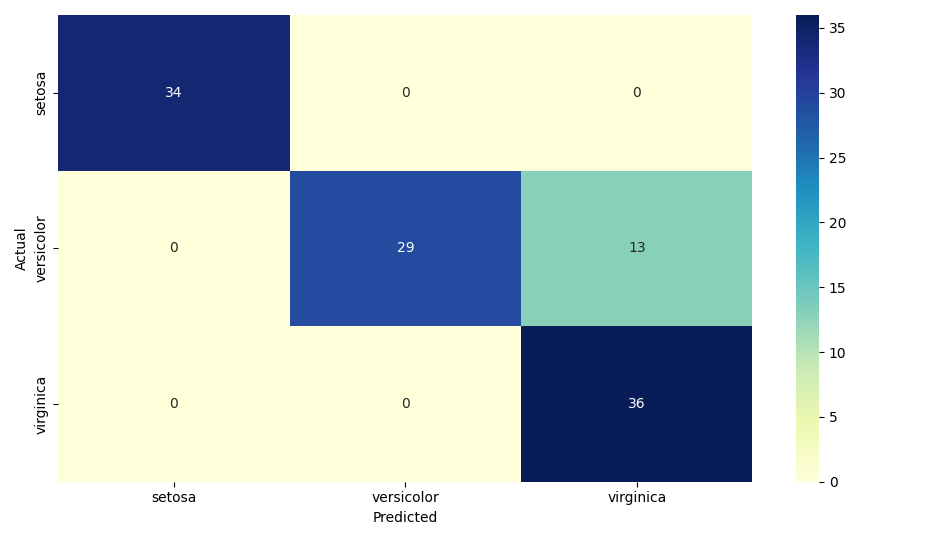
\includegraphics[width=\textwidth]{imagens/confusion_classic_train_en.png}
\smallcaption{Source: Author.}
\label{fig:matriz_confusao_classico_treino}
\end{figure}

\begin{table}[H]
\centering
\caption{Test results for the classical classifier.}
\small
\begin{tabular}{|c|c|c|c|}
\hline
\textbf{Metric} & \textbf{Setosa} & \textbf{Versicolor} & \textbf{Virginica} \\ \hline
Precision (Test) & 100.00\% & 87.50\% & 92.86\% \\ \hline
Recall (Test) & 100.00\% & 87.50\% & 92.86\% \\ \hline
F1-score (Test) & 100.00\% & 87.50\% & 92.86\% \\ \hline
Accuracy (Test) & \multicolumn{3}{|c|}{94.74\%} \\ \hline
Specificity (Test) & \multicolumn{3}{|c|}{97.50\%} \\ \hline
\end{tabular}
\smallcaption{Source: Author.}
\end{table}

\begin{figure}[H]
\centering
\caption{Test confusion matrix for the classical classifier.}
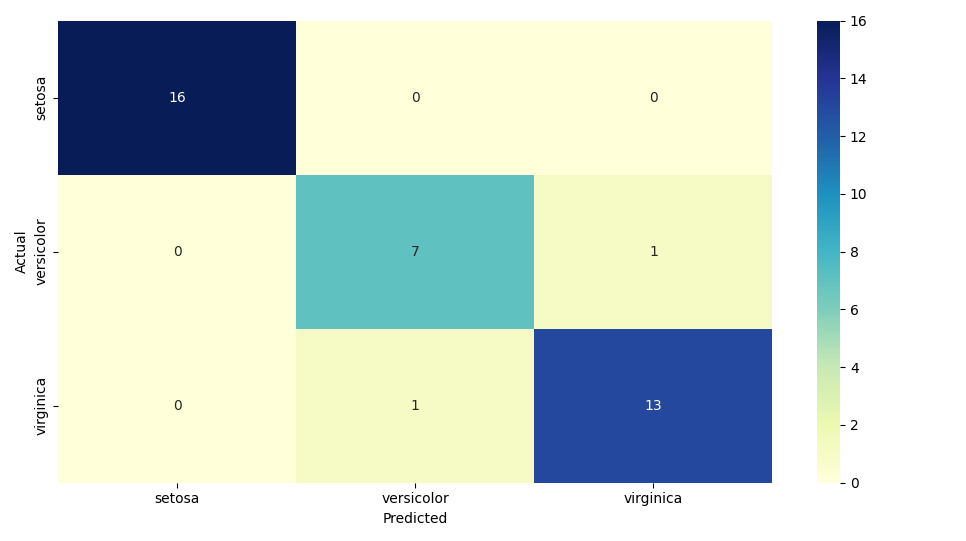
\includegraphics[width=\textwidth]{imagens/confusion_classic_test_en.png}
\smallcaption{Source: Author.}
\label{fig:matriz_confusao_classico_teste}
\end{figure}

\subsection{Quantum Classifier}

\begin{table}[H]
\centering
\caption{Training results for the quantum classifier.}
\small
\begin{tabular}{|c|c|c|c|}
\hline
\textbf{Metric} & \textbf{Setosa} & \textbf{Versicolor} & \textbf{Virginica} \\ \hline
Precision (Training) & 94.44\% & 70.59\% & 84.00\% \\ \hline
Recall (Training) & 100.00\% & 85.71\% & 58.33\% \\ \hline
F1-score (Training) & 97.14\% & 77.42\% & 68.85\% \\ \hline
Accuracy (Training) & \multicolumn{3}{|c|}{81.25\%} \\ \hline
Specificity (Training) & \multicolumn{3}{|c|}{90.24\%} \\ \hline
\end{tabular}
\smallcaption{Source: Author.}
\end{table}

\begin{figure}[H]
\centering
\caption{Training confusion matrix for the quantum classifier.}
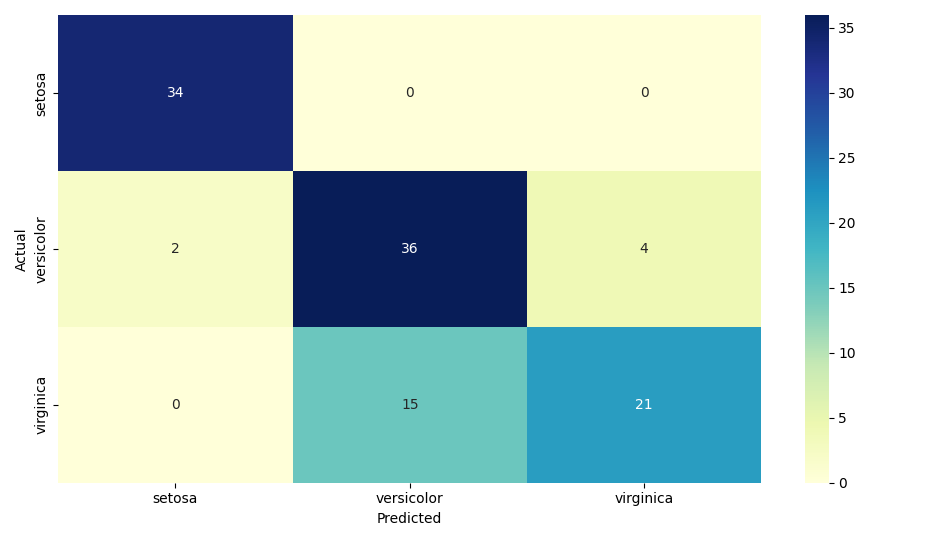
\includegraphics[width=\textwidth]{imagens/confusion_quantum_train_en.png}
\smallcaption{Source: Author.}
\label{fig:matriz_confusao_quantico_treino}
\end{figure}

\begin{table}[H]
\centering
\caption{Test results for the quantum classifier.}
\small
\begin{tabular}{|c|c|c|c|}
\hline
\textbf{Metric} & \textbf{Setosa} & \textbf{Versicolor} & \textbf{Virginica} \\ \hline
Precision (Test) & 94.12\% & 53.85\% & 100.00\% \\ \hline
Recall (Test) & 100.00\% & 87.50\% & 57.14\% \\ \hline
F1-score (Test) & 96.97\% & 66.67\% & 72.73\% \\ \hline
Accuracy (Test) & \multicolumn{3}{|c|}{81.58\%} \\ \hline
Specificity (Test) & \multicolumn{3}{|c|}{91.82\%} \\ \hline
\end{tabular}
\smallcaption{Source: Author.}
\end{table}

\begin{figure}[H]
\centering
\caption{Test confusion matrix for the quantum classifier.}
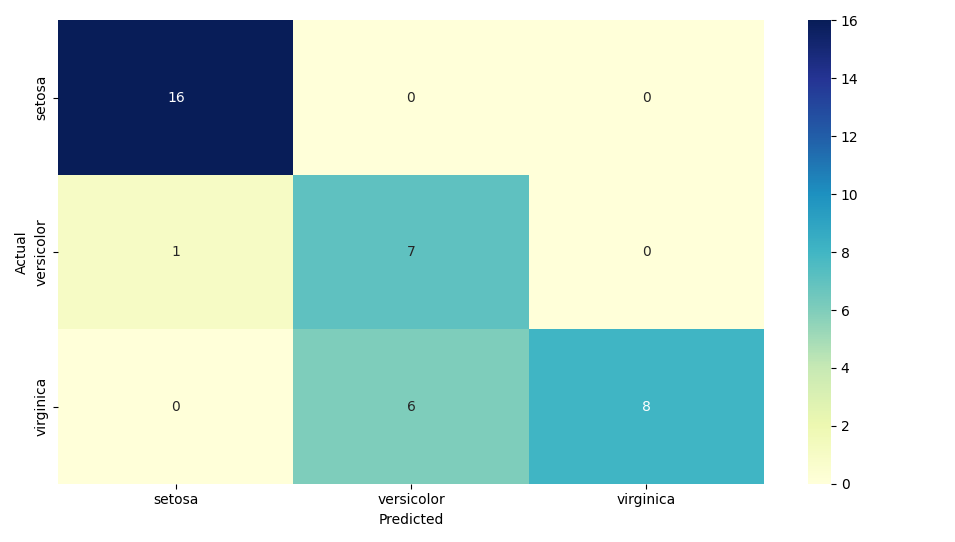
\includegraphics[width=\textwidth]{imagens/confusion_quantum_test_en.png}
\smallcaption{Source: Author.}
\label{fig:matriz_confusao_quantico_teste}
\end{figure}

% Number of parameters
It is important to note, however, that the model produced by the classical classifier had 584 parameters (146 support vectors with four components each, summed over the three one-vs-rest classifiers and corresponding to 89 distinct training samples), whereas the model produced by the quantum classifier had only 12 parameters, which are the angles of the twelve rotation gates in the \textit{ansatz}. The two quantities, however, are of different natures: the number of retained support vectors depends on the size of the training set and on the regularization parameter, whereas the twelve angles are fixed by the architecture of the circuit, regardless of the amount of data.

\subsection{Discussion of the Results}

Comparing the results obtained, the classical and quantum classifiers can be seen to have similar performance, although the classical classifier generally achieved greater accuracy. Specifically, the classical classifier achieved an accuracy of 88.39\% on the training set and 94.74\% on the test set, whereas the quantum classifier achieved an accuracy of 81.25\% on the training set and 81.58\% on the test set.

An important difference to highlight is the training time. The classical classifier took only 0.009 seconds to train, whereas the quantum classifier took 70.57 seconds. The two times, however, are not directly comparable: the classical classifier solves a quadratic optimization problem over the data, whereas the time of the quantum classifier includes building and executing the circuits at each COBYLA iteration. Even so, training time is an important aspect to consider when selecting a classifier, especially in situations in which that time is a critical factor.

With respect to precision, recall, and F1-score, both classifiers performed satisfactorily in most cases. However, there are some notable differences. For the \textit{Setosa} class, both classifiers achieved excellent results, with precision and recall of 100\% in most cases. For the \textit{Versicolor} and \textit{Virginica} classes, however, the classical classifier generally outperformed the quantum classifier.

These results suggest that, although the quantum classifier may be a valuable and promising tool for classification problems, challenges remain, especially in terms of time efficiency and performance on classes that are more difficult to classify. Further research is required to optimize the performance of the quantum classifier. During the performance-evaluation phase, the area under the ROC curves (AUC-ROC) was also used as a metric for evaluating the models:

\begin{figure}[H]
\centering
\caption{Training ROC curves for the classical and quantum classifiers.}
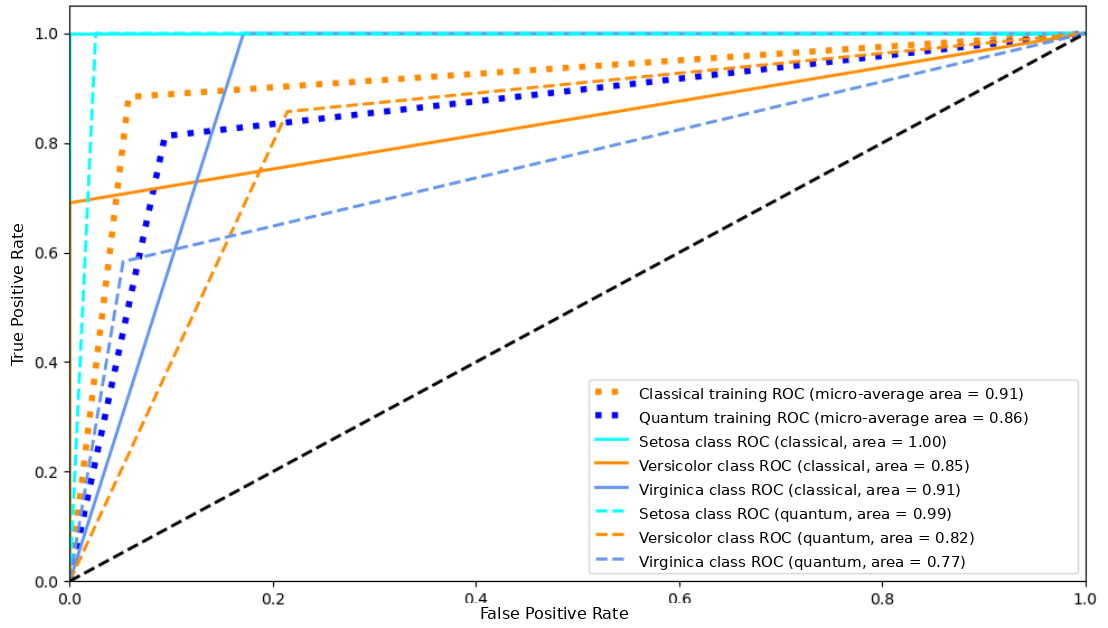
\includegraphics[width=\textwidth]{imagens/roc_train_en.png}
\smallcaption{Source: Author.}
\label{fig:roc_train}
\end{figure}

Receiver operating characteristic (ROC) curves are used to evaluate the performance of a classification model by plotting the true-positive rate as a function of the false-positive rate. The area under the curve (AUC) measures how well a model can distinguish between classes.

In Figure \ref{fig:roc_train}, the training ROC curve for the classical classifier had a micro-average area of 0.91, whereas the quantum classifier had a micro-average area of 0.86. For the \textit{Setosa} class, both approaches performed well, with an area of 1.00 for the classical classifier and 0.99 for the quantum classifier. For the \textit{Versicolor} and \textit{Virginica} classes, however, the classical classifier performed better, with areas of 0.85 and 0.91, respectively, compared with 0.82 and 0.77 for the quantum classifier.

\begin{figure}[H]
\centering
\caption{Test ROC curves for the classical and quantum classifiers.}
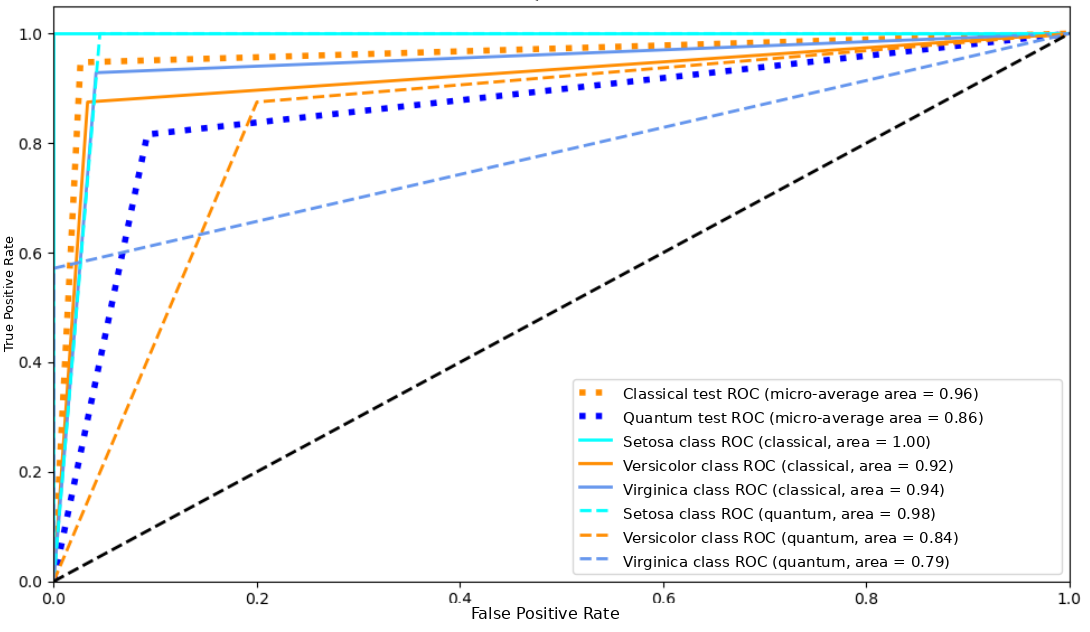
\includegraphics[width=\textwidth]{imagens/roc_test_en.png}
\smallcaption{Source: Author.}
\label{fig:roc_test}
\end{figure}

Figure \ref{fig:roc_test} presents the test ROC curves for the classical and quantum classifiers. The classical classifier obtained a micro-average area of 0.96, whereas the quantum classifier obtained a micro-average area of 0.86. Both approaches were effective in classifying the \textit{Setosa} class, with an area of 1.00 for the classical classifier and 0.98 for the quantum classifier. For the \textit{Versicolor} and \textit{Virginica} classes, the classical classifier performed better, with areas of 0.92 and 0.94, respectively, whereas the quantum classifier had areas of 0.84 and 0.79.

It is important to note that these ROC curves and AUC values are only one of the many aspects to consider when evaluating classifier performance. The nature of the problem, the importance of false positives versus false negatives, the distribution of the classes, and other factors must also be taken into account.

These results corroborate the previous discussion: the classical classifier performs slightly better than the quantum classifier in most cases, although both are effective at distinguishing between the classes. The effectiveness of the quantum classifier is particularly notable given the relative novelty of quantum computing and its potential for future improvements.


In summary, this study compared the performance of classical and quantum classifiers in classifying the Iris dataset. The results indicate that both classifiers are effective, with the classical classifier performing slightly better. Nevertheless, the effectiveness of the quantum classifier demonstrates the considerable potential of quantum computing in machine learning.

\section{Evaluation of Classifier Behavior as a Function of Training-Set Size}

This section evaluates the behavior of the classical and quantum classifiers as a function of training-set size. Several performance metrics were evaluated, including accuracy, specificity, recall, F1-score, and AUC-ROC. Each metric was evaluated for different training-set sizes, ranging from 20\% to 80\% of the complete dataset. The results are presented below in four tables, each corresponding to one classifier and one training or test split.

\begin{table}[H]
\centering
\caption{Classical-classifier training metrics for different training-set sizes.}
\small
\begin{tabular}{|c|c|c|c|c|c|c|}
\hline
\textbf{Training Size} & \textbf{Accuracy} & \textbf{Specificity} & \textbf{Recall} & \textbf{F1-score} & \textbf{AUC-ROC} \\ \hline
20\% & 63.3\% & 79.6\% & 63.3\% & 63.3\% & 73.1\% \\ \hline
30\% & 84.4\% & 91.8\% & 84.4\% & 84.4\% & 89.6\% \\ \hline
40\% & 85.0\% & 92.5\% & 85.0\% & 85.0\% & 89.6\% \\ \hline
50\% & 88.0\% & 94.1\% & 88.0\% & 88.0\% & 91.7\% \\ \hline
60\% & 82.2\% & 91.4\% & 82.2\% & 82.2\% & 87.9\% \\ \hline
70\% & 87.6\% & 94.0\% & 87.6\% & 87.6\% & 91.6\% \\ \hline
80\% & 88.3\% & 94.2\% & 88.3\% & 88.3\% & 91.8\% \\ \hline
\end{tabular}
\smallcaption{Source: Author.}
\end{table}

\begin{table}[H]
\centering
\caption{Classical-classifier test metrics for different training-set sizes.}
\small
\begin{tabular}{|c|c|c|c|c|c|c|}
\hline
\textbf{Training Size} & \textbf{Accuracy} & \textbf{Specificity} & \textbf{Recall} & \textbf{F1-score} & \textbf{AUC-ROC} \\ \hline
20\% & 73.3\% & 87.1\% & 73.3\% & 73.3\% & 79.9\% \\ \hline
30\% & 86.7\% & 93.4\% & 86.7\% & 86.7\% & 89.2\% \\ \hline
40\% & 91.1\% & 95.5\% & 91.1\% & 91.1\% & 92.7\% \\ \hline
50\% & 96.0\% & 98.0\% & 96.0\% & 96.0\% & 96.7\% \\ \hline
60\% & 91.7\% & 95.6\% & 91.7\% & 91.7\% & 92.6\% \\ \hline
70\% & 95.6\% & 97.9\% & 95.6\% & 95.6\% & 96.3\% \\ \hline
80\% & 96.7\% & 98.2\% & 96.7\% & 96.7\% & 96.3\% \\ \hline
\end{tabular}
\smallcaption{Source: Author.}
\end{table}

\begin{table}[H]
\centering
\caption{Quantum-classifier training metrics for different training-set sizes.}
\small
\begin{tabular}{|c|c|c|c|c|c|c|}
\hline
\textbf{Training Size} & \textbf{Accuracy} & \textbf{Specificity} & \textbf{Recall} & \textbf{F1-score} & \textbf{AUC-ROC} \\ \hline
20\% & 76.7\% & 86.3\% & 76.7\% & 76.7\% & 82.5\% \\ \hline
30\% & 80.0\% & 88.5\% & 80.0\% & 80.0\% & 84.9\% \\ \hline
40\% & 81.7\% & 89.8\% & 81.7\% & 81.7\% & 85.3\% \\ \hline
50\% & 74.7\% & 86.0\% & 74.7\% & 74.7\% & 78.8\% \\ \hline
60\% & 70.0\% & 84.0\% & 70.0\% & 70.0\% & 76.2\% \\ \hline
70\% & 73.3\% & 85.8\% & 73.3\% & 73.3\% & 78.9\% \\ \hline
80\% & 80.0\% & 89.6\% & 80.0\% & 80.0\% & 84.7\% \\ \hline
\end{tabular}
\smallcaption{Source: Author.}
\end{table}

\begin{table}[H]
\centering
\caption{Quantum-classifier test metrics for different training-set sizes.}
\small
\begin{tabular}{|c|c|c|c|c|c|c|}
\hline
\textbf{Training Size} & \textbf{Accuracy} & \textbf{Specificity} & \textbf{Recall} & \textbf{F1-score} & \textbf{AUC-ROC} \\ \hline
20\% & 74.2\% & 87.4\% & 74.2\% & 74.2\% & 81.1\% \\ \hline
30\% & 80.0\% & 90.5\% & 80.0\% & 80.0\% & 85.0\% \\ \hline
40\% & 75.6\% & 88.5\% & 75.6\% & 75.6\% & 82.4\% \\ \hline
50\% & 69.3\% & 85.9\% & 69.3\% & 69.3\% & 78.8\% \\ \hline
60\% & 61.7\% & 82.3\% & 61.7\% & 61.7\% & 73.2\% \\ \hline
70\% & 66.7\% & 85.1\% & 66.7\% & 66.7\% & 76.5\% \\ \hline
80\% & 83.3\% & 93.1\% & 83.3\% & 83.3\% & 89.0\% \\ \hline
\end{tabular}
\smallcaption{Source: Author.}
\end{table}

\subsection{Discussion of the Results}

Analysis of the results shows that, in general, the classical classifier outperformed the quantum classifier for most metrics across all training-set sizes. This suggests that the classical model may be more suitable for this dataset.

However, the quantum classifier also performed consistently across all metrics and training-set sizes, which indicates its robustness. With further optimization, the quantum classifier may match or even exceed the performance of the classical classifier. Therefore, the applicability and effectiveness of quantum classifiers require further study.

\section{Results of the Comparison Tests on a Real Quantum Computer}

\begin{table}[H]
\centering
\caption{Training results for the classical classifier.}
\small
\begin{tabular}{|c|c|c|c|}
\hline
\textbf{Metric} & \textbf{Setosa} & \textbf{Versicolor} & \textbf{Virginica} \\ \hline
Precision (Training) & 100.00\% & 89.74\% & 94.29\% \\ \hline
Recall (Training) & 100.00\% & 94.59\% & 89.19\% \\ \hline
F1-score (Training) & 100.00\% & 92.11\% & 91.67\% \\ \hline
Accuracy (Training) & \multicolumn{3}{|c|}{94.29\%} \\ \hline
\end{tabular}
\smallcaption{Source: Author.}
\end{table}

\begin{table}[H]
\centering
\caption{Test results for the classical classifier.}
\small
\begin{tabular}{|c|c|c|c|}
\hline
\textbf{Metric} & \textbf{Setosa} & \textbf{Versicolor} & \textbf{Virginica} \\ \hline
Precision (Test) & 100.00\% & 100.00\% & 100.00\% \\ \hline
Recall (Test) & 100.00\% & 100.00\% & 100.00\% \\ \hline
F1-score (Test) & 100.00\% & 100.00\% & 100.00\% \\ \hline
Accuracy (Test) & \multicolumn{3}{|c|}{100.00\%} \\ \hline
\end{tabular}
\smallcaption{Source: Author.}
\end{table}

%\begin{figure}[H]
%\centering
%\caption{Test confusion matrix for the classical classifier.}
%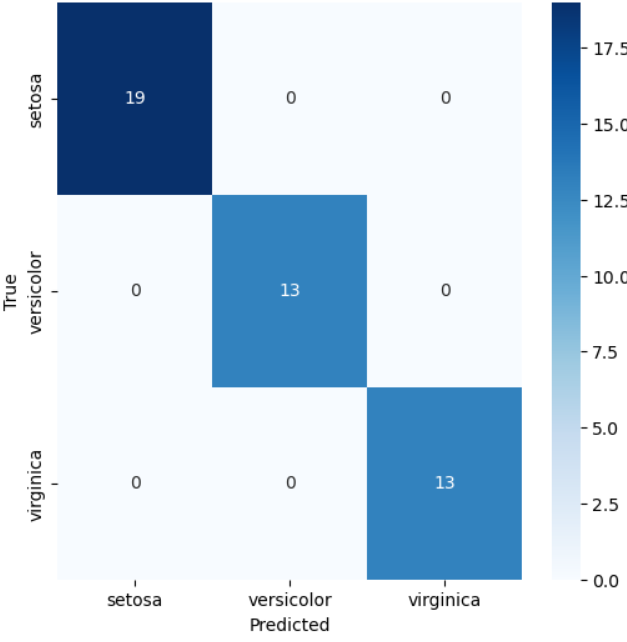
\includegraphics[width=.7\textwidth]{imagens/confusion_classic_test_real.png}
%\subcaption*{Source: Author.}
%\label{fig:matriz_confusao_classico_teste_real}
%\end{figure}

\begin{table}[H]
\centering
\caption{Training results for the quantum classifier.}
\small
\begin{tabular}{|c|c|c|c|}
\hline
\textbf{Metric} & \textbf{Setosa} & \textbf{Versicolor} & \textbf{Virginica} \\ \hline
Precision (Training) & 67.39\% & 45.28\% & 100.00\% \\ \hline
Recall (Training) & 100.00\% & 64.86\% & 16.22\% \\ \hline
F1-score (Training) & 80.52\% & 53.33\% & 27.91\% \\ \hline
Accuracy (Training) & \multicolumn{3}{|c|}{58.10\%} \\ \hline
\end{tabular}
\smallcaption{Source: Author.}
\end{table}

\begin{table}[H]
\centering
\caption{Test results for the quantum classifier.}
\small
\begin{tabular}{|c|c|c|c|}
\hline
\textbf{Metric} & \textbf{Setosa} & \textbf{Versicolor} & \textbf{Virginica} \\ \hline
Precision (Test) & 90.48\% & 52.17\% & 100.00\% \\ \hline
Recall (Test) & 100.00\% & 92.31\% & 7.69\% \\ \hline
F1-score (Test) & 95.00\% & 66.67\% & 14.29\% \\ \hline
Accuracy (Test) & \multicolumn{3}{|c|}{71.11\%} \\ \hline
\end{tabular}
\smallcaption{Source: Author.}
\end{table}

%\begin{figure}[H]
%\centering
%\caption{Test confusion matrix for the real quantum classifier.}
%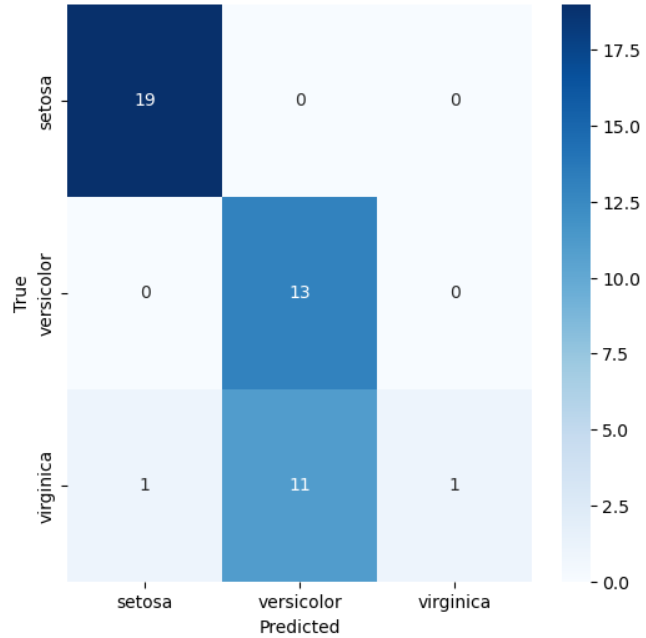
\includegraphics[width=.7\textwidth]{imagens/confusion_quantum_test_real.png}
%\subcaption*{Source: Author.}
%\label{fig:matriz_confusao_quantico_teste_real}
%\end{figure}

\subsection{Discussion of the Results}

This section discusses the results obtained by the quantum classifier, taking into account the limitations and configurations used.

The quantum classifier was trained with specific configurations, including only one repetition of \textit{ZFeatureMap}, one repetition of \textit{RealAmplitudes}, and only 20 COBYLA iterations, which may mean that the model optimization was incomplete. In addition, 70\% of the dataset was used as the training set, which corresponds to 105 training samples and 45 test samples. These configurations may affect the performance of the quantum classifier, limiting it in comparison with the classical classifier.

Analysis of the results shows that the quantum classifier performed worse than the classical classifier for all evaluated metrics. On the training set, the accuracy of the quantum model was 58.10\%, whereas on the test set it was 71.11\%. This difference does not indicate better generalization: the two samples differ in composition, since the \textit{Setosa} class, the only one classified correctly in every case, accounts for 42.2\% of the test set and 29.5\% of the training set, whereas the \textit{Virginica} class, the one with the lowest \textit{recall}, accounts for 28.9\% and 35.2\%, respectively. Reweighting the per-class \textit{recall} obtained on the test set by the class proportions of the training set, the test accuracy would correspond to 64.76\%, and the remaining difference is not statistically significant at these sample sizes (Fisher's exact test, $p = 0.15$).

In addition, the precision, recall, and F1-score metrics were also lower for the quantum classifier than for the classical classifier. Precision was 90.48\% for the \textit{Setosa} class, 52.17\% for \textit{Versicolor}, and 100.00\% for \textit{Virginica}. Recall was 100.00\% for \textit{Setosa}, 92.31\% for \textit{Versicolor}, and 7.69\% for \textit{Virginica}. The F1-score was 95.00\% for \textit{Setosa}, 66.67\% for \textit{Versicolor}, and 14.29\% for \textit{Virginica}.

These results indicate that, with the configurations used and the limited amount of training data, the quantum classifier was unable to capture the patterns in the data effectively. It is important to emphasize that the performance of the quantum classifier can be improved by adjusting the configurations, such as increasing the number of \textit{ZFeatureMap} and \textit{RealAmplitudes} repetitions, increasing the number of COBYLA iterations, and using a larger proportion of the dataset for training.

Therefore, under the configurations used in this study, the quantum classifier performed below the classical classifier. However, it is important to emphasize that quantum computing is still in the early stages of development and improvement. As quantum technology advances and research in this area continues, quantum classifiers are expected to overcome current limitations and provide increasingly promising results for complex classification tasks.